\section{Test Interaction Region}

The main interaction region assembly is several meters long and consists of
delicate glass-plate electrodes which have to be aligned very precisely before
they can be used in the experiment. In order to allow testing of the entire
beamline before the interaction region is fully assembled, we have decided to
make a scaled-down model of if, described in this section.

\subsection{Vacuum chamber}

The vacuum chamber is a glass tube (252~mm ID, 260~mm OD, 900~mm long, from
Technical Glass Products) with custom vacuum flanges fitted at each end. The
flanges are the same pieces that will be used with the full-scale vacuum
chamber. Testing with helium revealed no leaks at the flanges.

\subsection{Electrode assembly}

The two electrodes (Fig.~\ref{test_elec}) were machined out of grade 5 titanium
by Xometry and polished to a mirror finish (best finish possible) by the Central
Electropolishing Company. (See ref. \cite{ready2021surface} for information
about surface conditioning of high-voltage electrodes.) The shape is exactly the
same as for the full-scale electrodes, except they have been shortened to
approx.\ 60~cm.

\begin{figure}
    \centering
    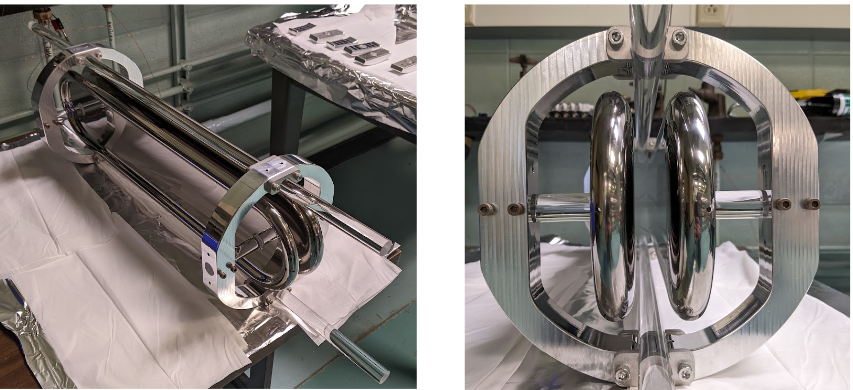
\includegraphics[width=\textwidth]{figs/todo/test_elec.png}
    \caption{Electrode assembly for the test interaction region before being
    placed in the vacuum chamber.}
    \label{test_elec}
\end{figure}

The electrodes are held in place inside the vacuum chamber by two aluminum
rings, each of which consists of two C-shaped pieces. The two pieces are bolted
together using a small aluminum connecting plate, which also contains a cutout
to hold a 20~mm glass rod (89~cm long) both above and below the two electrodes.
The glass rods can be used as rails to translate a sensor between the
electrodes, such as a magnetometer or a capacitive sensor to measure electrode
spacing as a function of position along the length of the electrodes.

Each electrode is attached to the rings using two short fused quartz rods (19~mm
diameter, 90.2~mm long) that are epoxied into a shallow blind hole at the back
of the electrodes. Since the epoxy joint is recessed into the electrode, it is
located very close to the center-of-mass line of each electrode, resulting in a
very low force acting to `peel off' the joint (Fig.~\ref{epoxy_forces}). After
comparing several types of epoxies (Table~\ref{epoxies}), we chose Torr Seal for
its excellent vacuum properties, common availability, and ease of use.

\begin{figure}
    \centering
    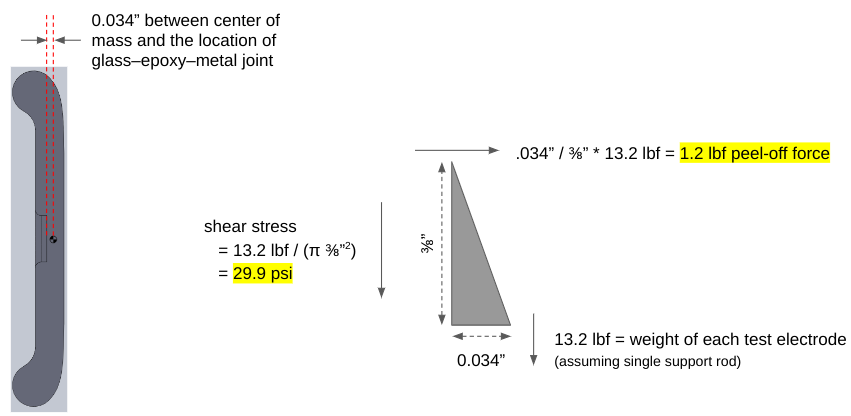
\includegraphics[width=\textwidth]{figs/todo/epoxy_forces.png}
    \caption{Forces acting on the epoxy joint holding the electrodes.}
    \label{epoxy_forces}
\end{figure}

\begin{table*}
  %\small
  \makebox[\textwidth][c]{%
    \begin{tabu} to \textwidth {rcc}
      \toprule
        & shear stress & peel-off force \\\midrule
        test interaction region  & 29.9 psi        & 1.2 pli\\
        10$\times$ safety factor & 299 psi         & 12 pli\\
        main interaction region  & 76.3 psi        & 15.6 pli total\\\midrule
        Master Bond Supreme 10HT & 3,600–3,800 psi & 25--30 pli\\
        Master Bond EP30-2       & 3,000–3,200 psi & not specified\\
        Torr Seal                & 2000 psi        & not specified\\
      \bottomrule
    \end{tabu}}
    \caption{A comparison of shear stress and peel-off force requirements and
    epoxy performance (from their respective datasheets).}
    \label{epoxies}
\end{table*}

\subsection{Magnetic shield}

The magnetic shield (Fig.~\ref{test_shield}) is constructed around a single
schedule 40 PVC pipe, 14" diameter, 4~ft long, which has been wrapped with two
layers of Co-netic foil, 0.254~mm thick. The foil comes in 15" wide sheets;
three such sheets (with 1" overlaps) were wrapped circumferentially around the
plastic tube. In addition, 12 turns of a degaussing wire were wrapped in a
toroidal fashion around the shield. The static residual field inside the shield
along the central axis is shown in Fig.~\ref{test_shield_field}.

\begin{figure}
    \centering
    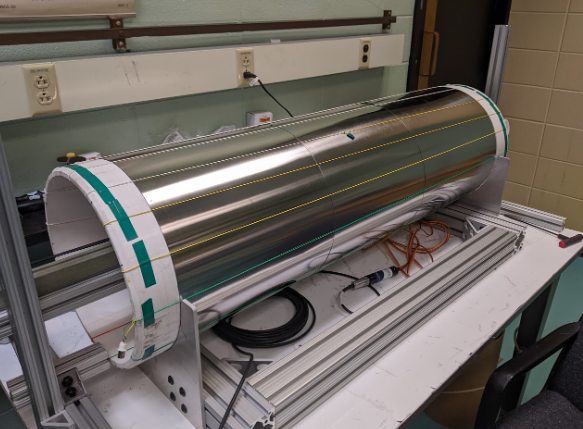
\includegraphics[width=.7\textwidth]{figs/todo/test_shield.png}
    \caption{Magnetic shield for test interaction region.}
    \label{test_shield}
\end{figure}

\begin{figure}
    \centering
    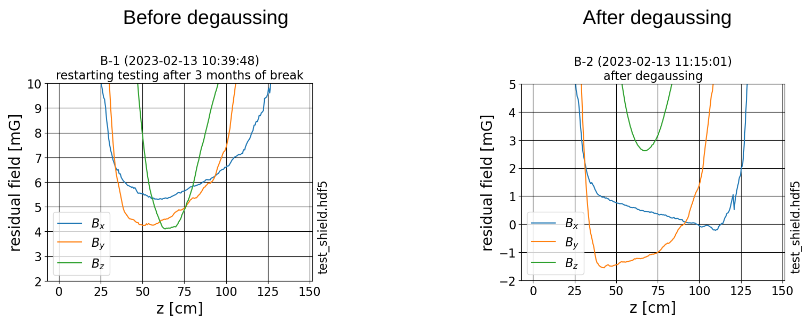
\includegraphics[width=\textwidth]{figs/todo/test_shield_data.png}
    \caption{Magnetic fields inside the test interaction region shield.}
    \label{test_shield_field}
\end{figure}
